% Appendix D

\chapter{Supplementary figures} % Main appendix title
\chaptermark{Supplementary figures}
\label{AppendixE} % For referencing this appendix elsewhere, use \ref{AppendixA}

%\lhead{Appendix C. \emph{Statistical Tests}} % This is for the header on each page - perhaps a shortened title

\section{Confusion matrix Chapter 2}

\begin{figure}[h!]
\centering
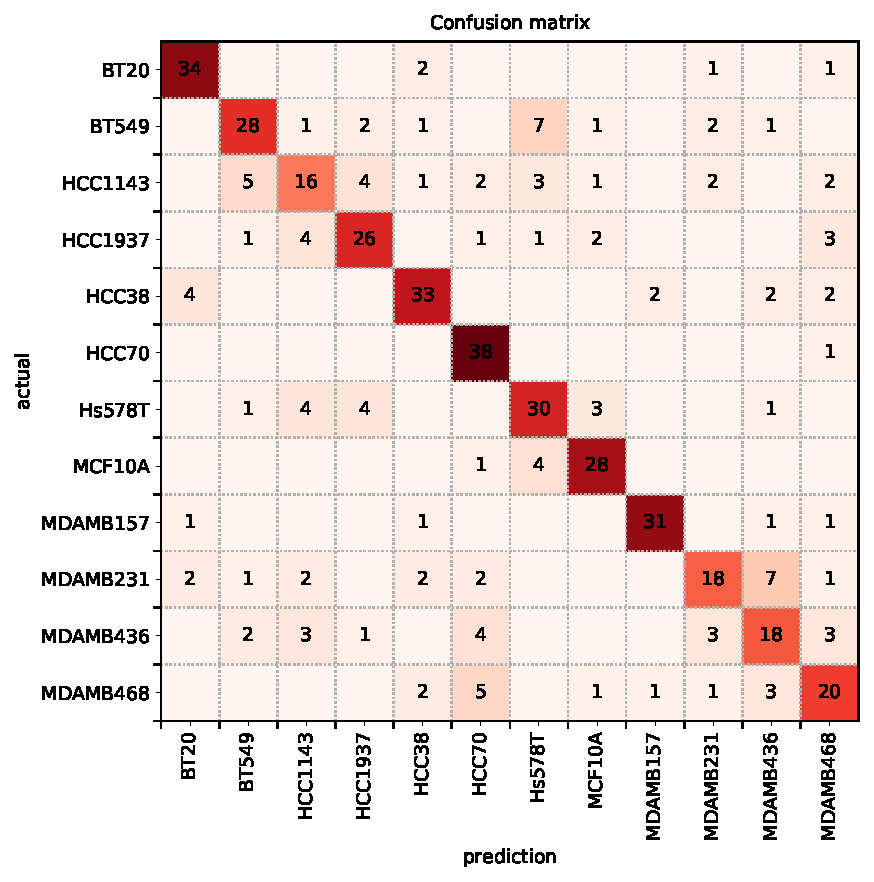
\includegraphics[width=0.8\textwidth]{img/confusion_matrix.pdf}
\caption{Viability comparison between cell lines for a variety of drugs and negative controls. The neutral DMSO and untreated wells strongly overlap, while showing considerable variation in both cell lines. Viability correlates well between cell lines with Pearson correlation coefficient $\rho = 0.6556$}
\label{fig:viability}
\end{figure}

\section{Differential drug effects Chapter 3}

\begin{figure}[!ht]
     \subfloat[Endothall takes effect in cell line MDA231 only.\label{subfig-1:dummy}]{%
       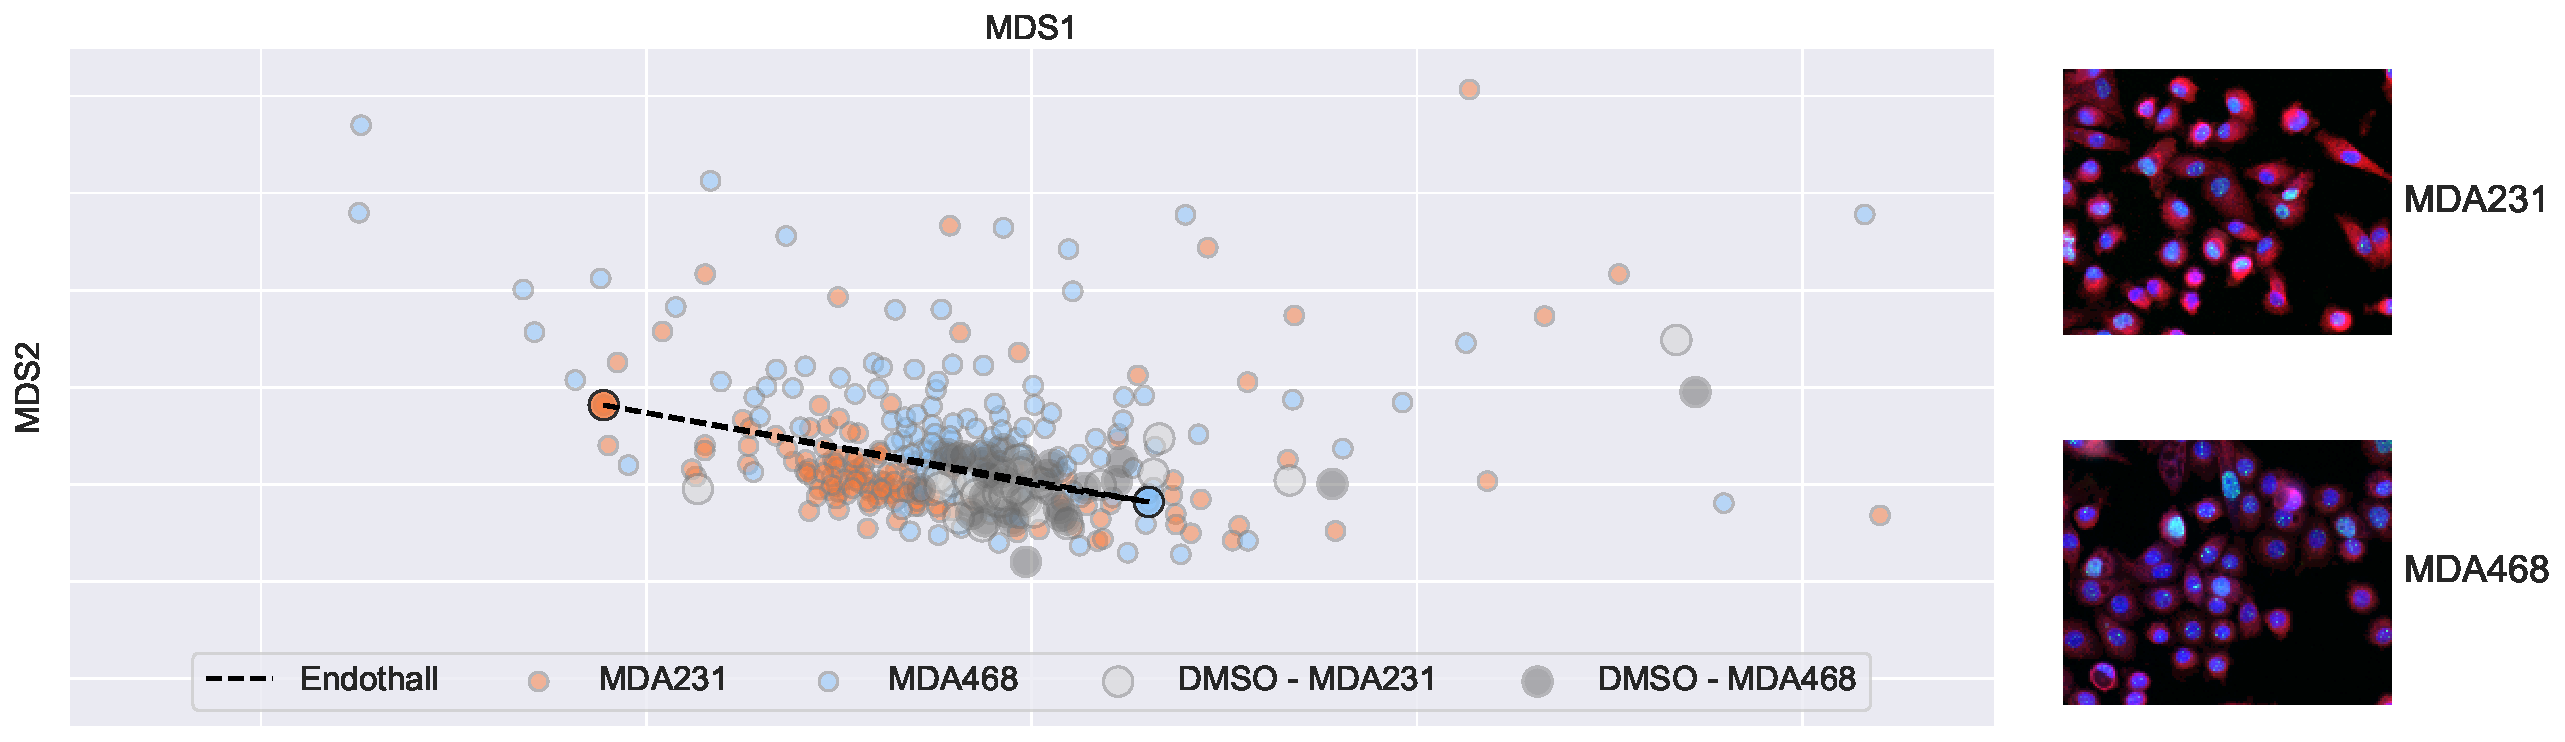
\includegraphics[width=\textwidth]{img/endothall.pdf}
     }
     \hfill
     \subfloat[CL-82198 takes effect in cell line MDA468 only.\label{subfig-2:dummy}]{%
       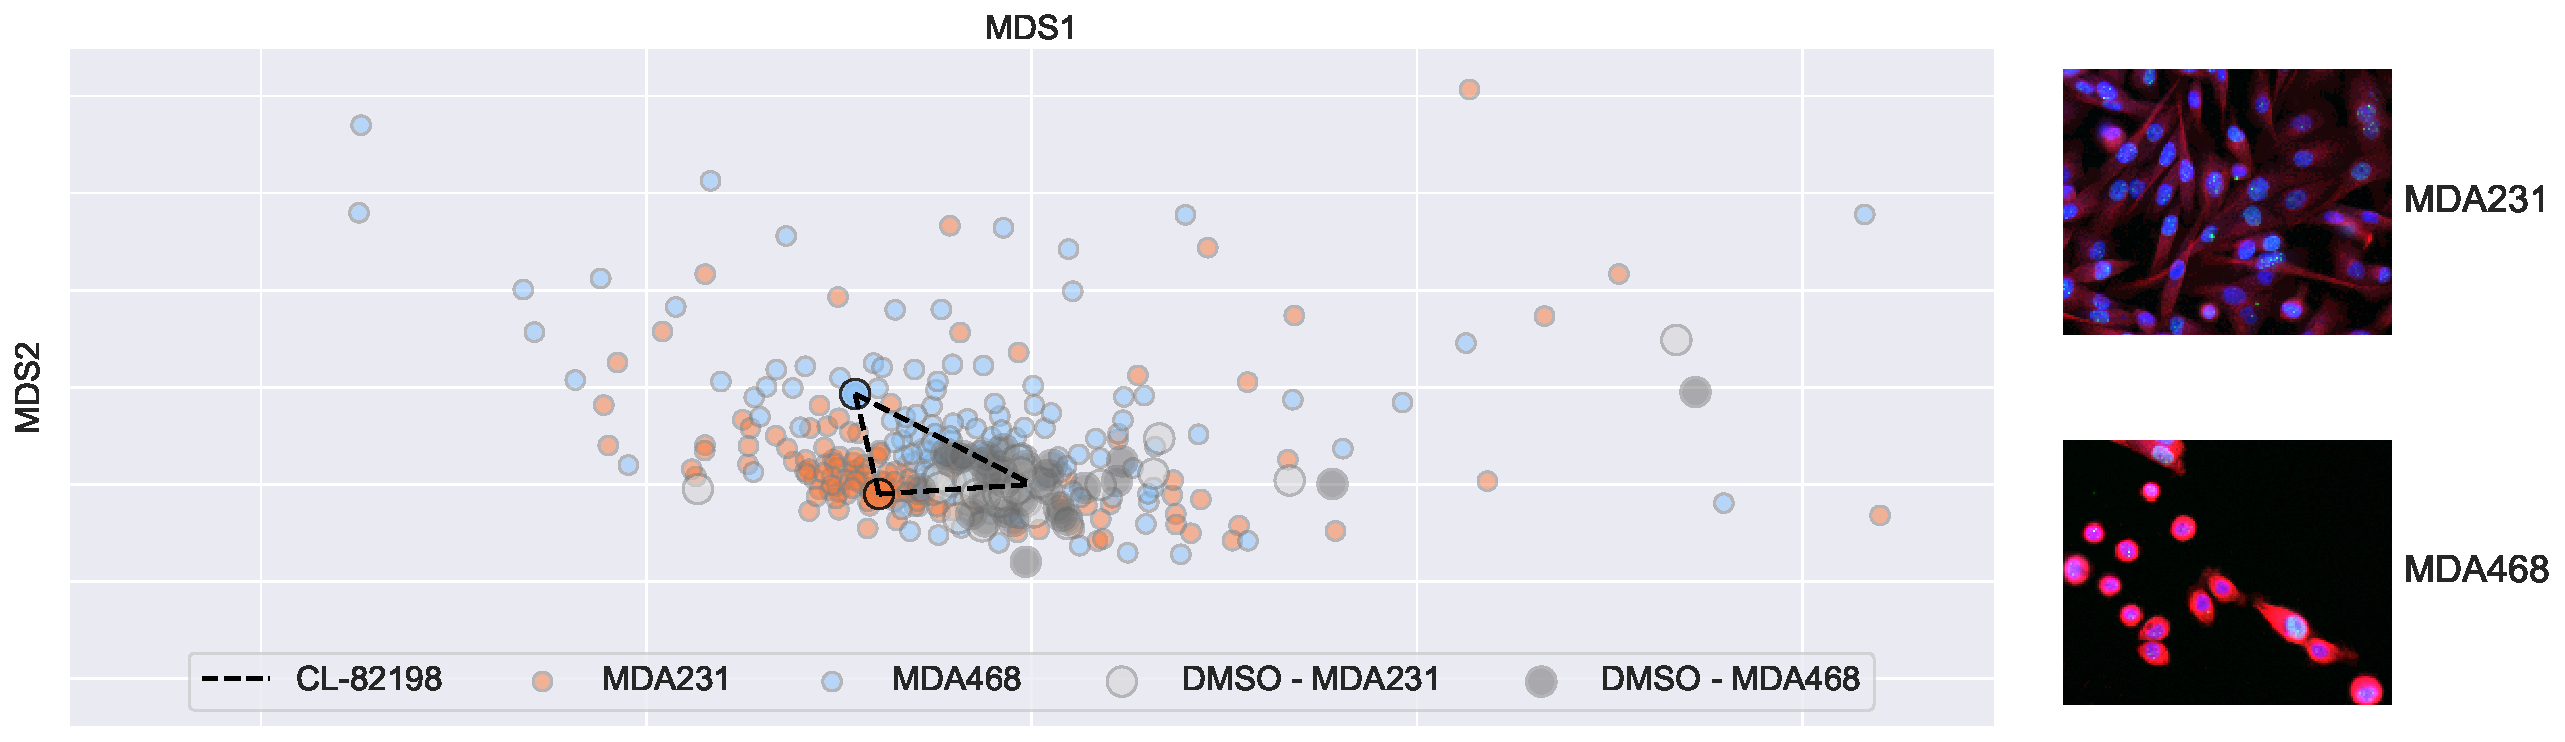
\includegraphics[width=\textwidth]{img/cl-82198.pdf}
     }
     \hfill
     \subfloat[Cyclosporin A takes a similar in both cell lines.\label{subfig-2:dummy}]{%
       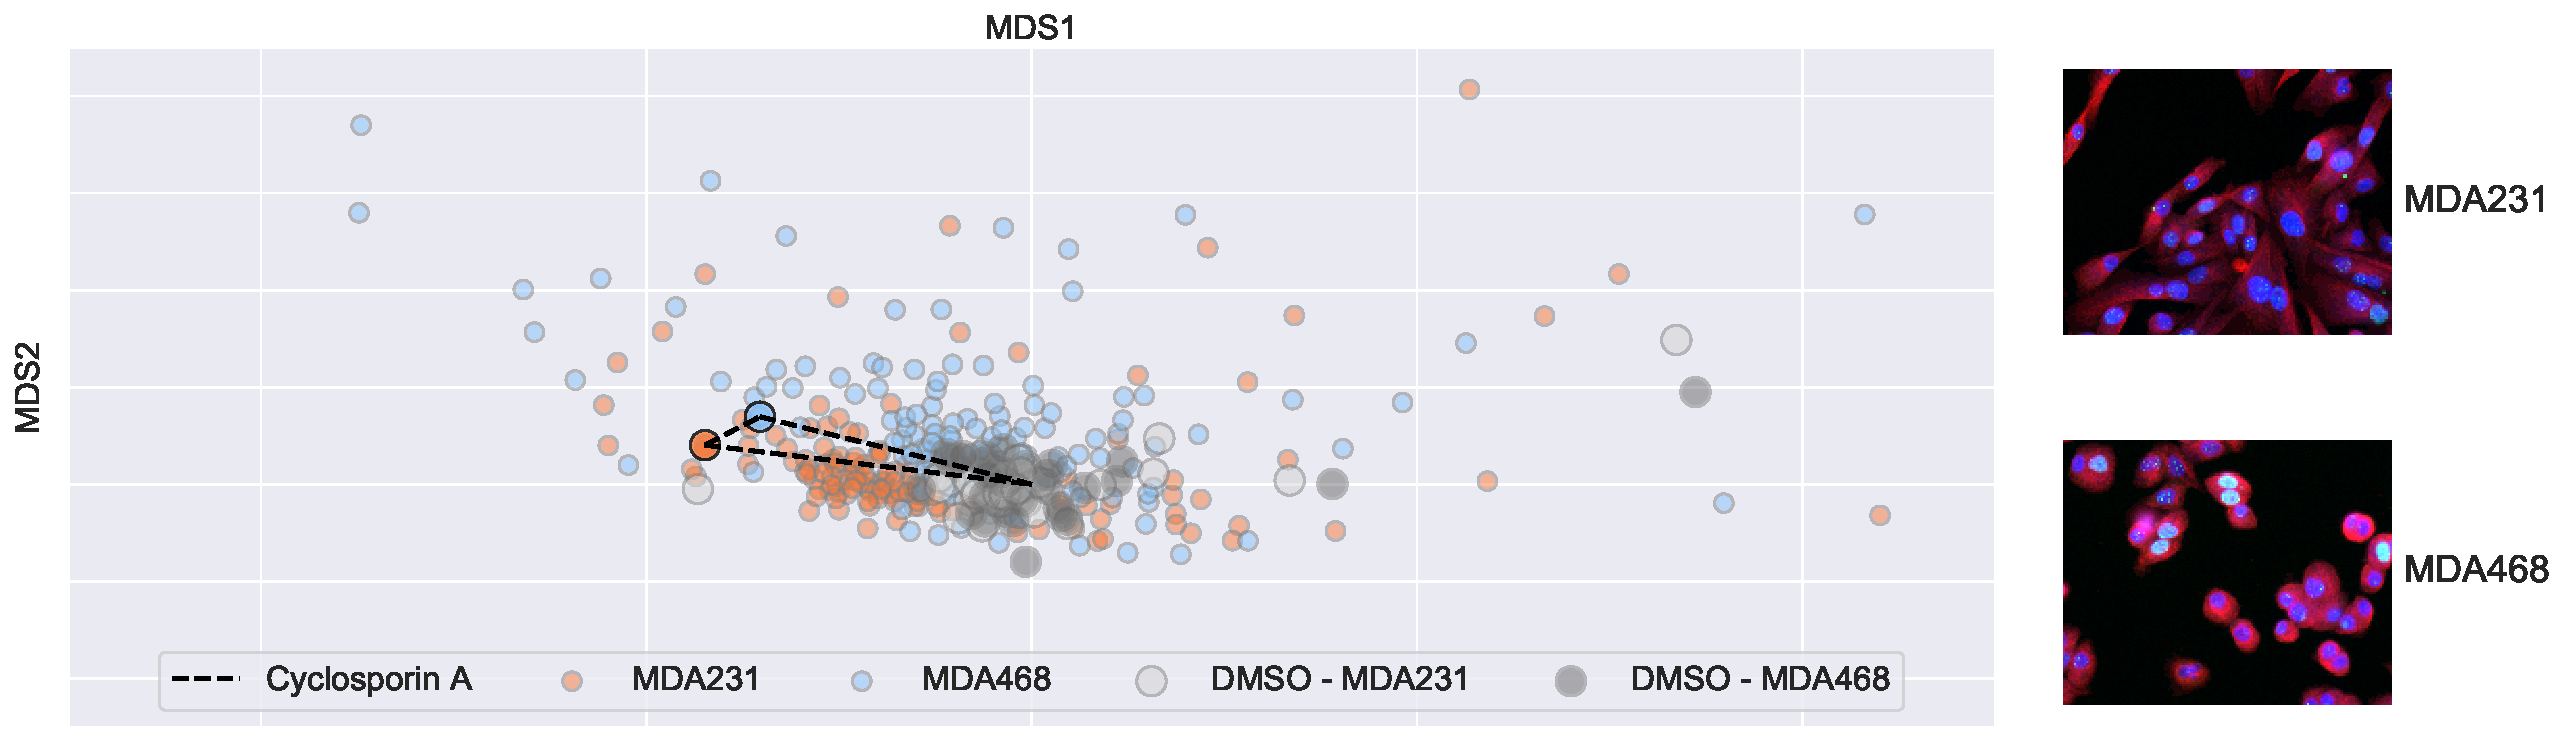
\includegraphics[width=\textwidth]{img/cyclosporin-A.pdf}
     }
     \hfill
     \subfloat[PKC-412 takes differential effects in the two cell lines.\label{subfig-2:dummy}]{%
       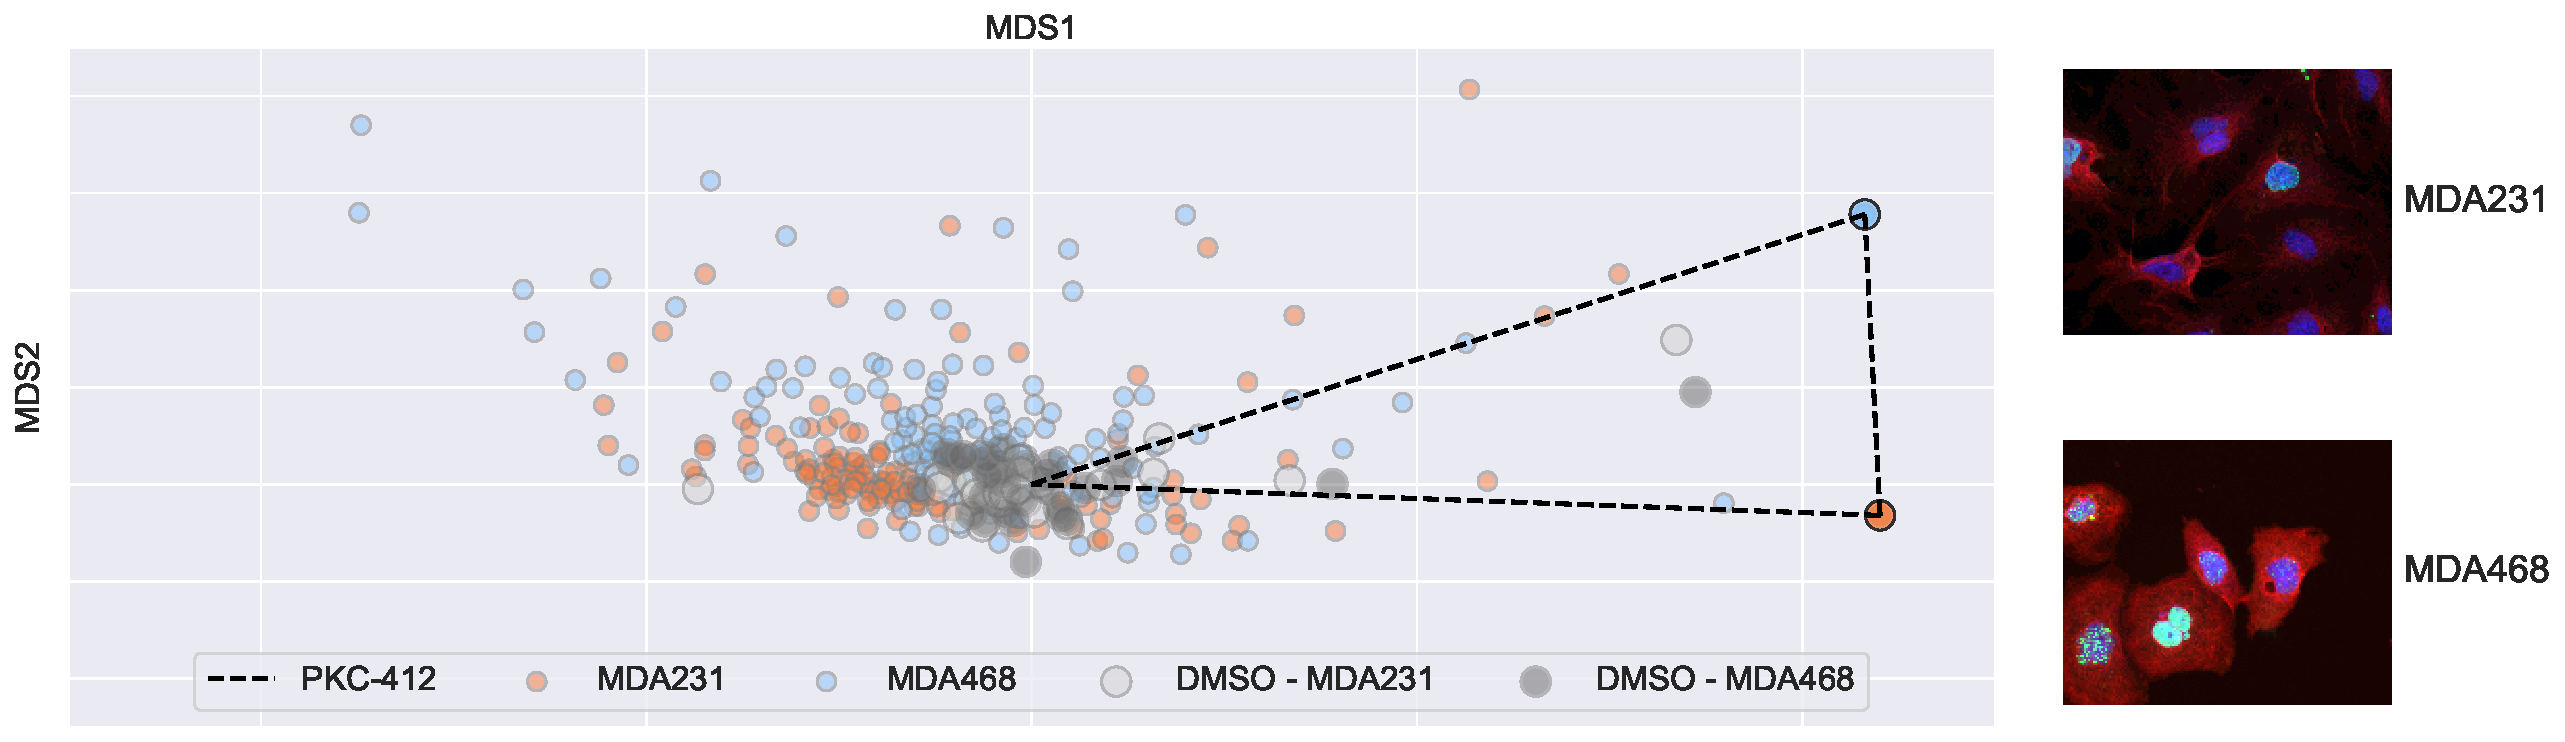
\includegraphics[width=\textwidth]{img/pkc-412.pdf}
     }
     \caption{MDS plots of each category of drug effect. The distances between the profiles are plotted as a line, as well as the respective distances to the centroid (origin).}
     \label{fig:dummy}
\end{figure}

\section{Biological phenomena Chapter 4}

\begin{figure}[h!]%
    \centering
    \subfloat[$t = 42$]{{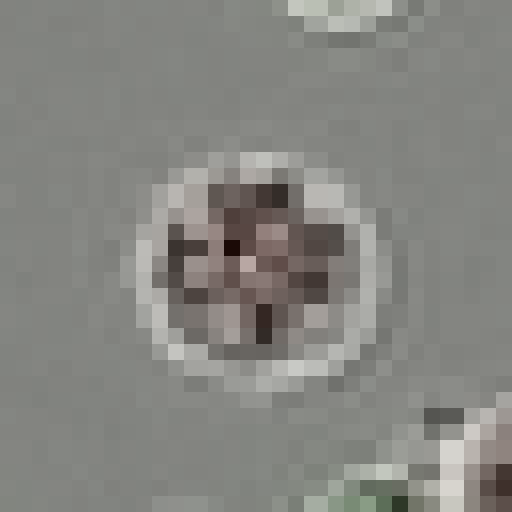
\includegraphics[width=0.25\textwidth]{img/r_t_cell_21.png}}}%
    \qquad
    \subfloat[$t = 44$]{{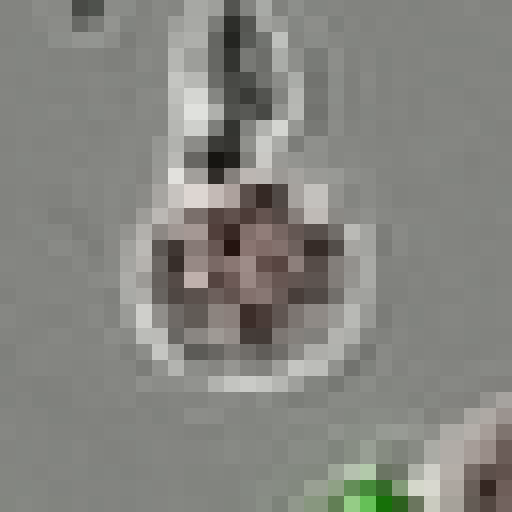
\includegraphics[width=0.25\textwidth]{img/r_t_cell_22.png}}}%
    \qquad
    \subfloat[$t = 92$]{{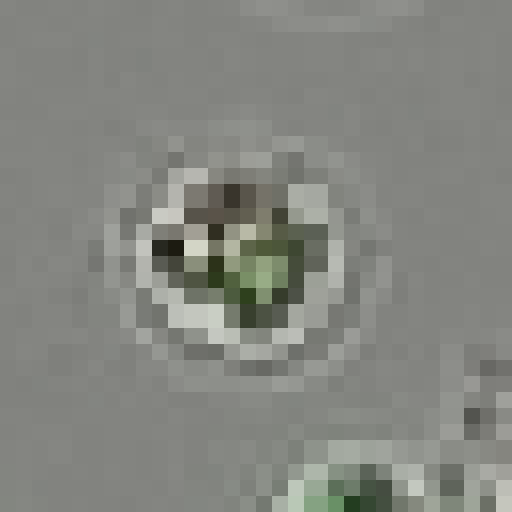
\includegraphics[width=0.25\textwidth]{img/r_t_cell_46.png}}}%
    \caption{An application of a neural algorithm of artistic style to phase contrast images of CAR-T cells (a) and a style source image (b) to synthesise a new image combining their characteristics in a ``simulated'' image (c).}%
    \label{fig:t_cell_latch}
\end{figure}

\begin{figure}[h!]%
    \centering
    \subfloat[$t = 42$]{{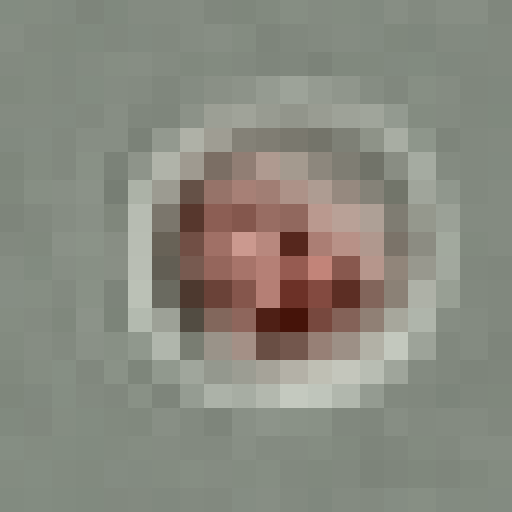
\includegraphics[width=0.25\textwidth]{img/r_dying_cell_0000.png}}}%
    \qquad
    \subfloat[$t = 44$]{{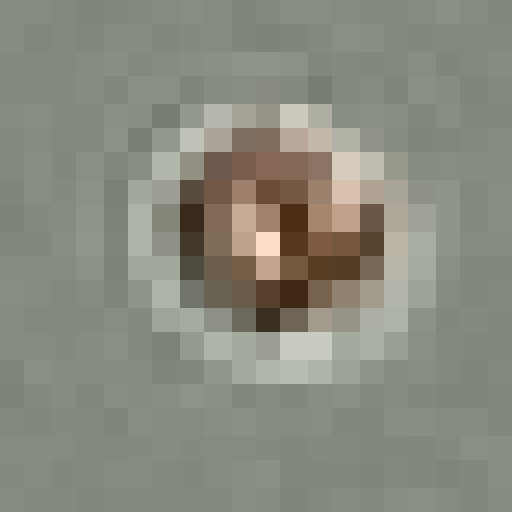
\includegraphics[width=0.25\textwidth]{img/r_dying_cell_0001.png}}}%
    \qquad
    \subfloat[$t = 92$]{{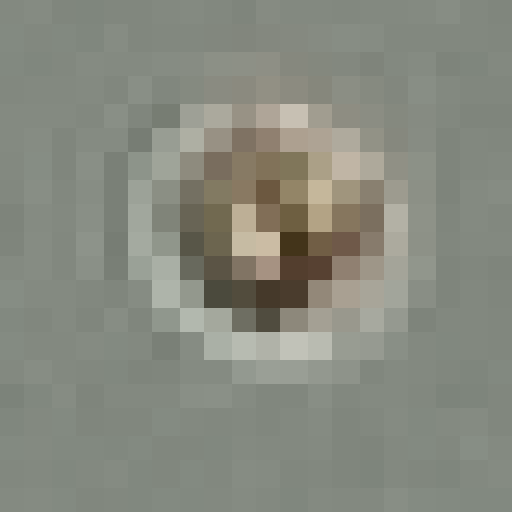
\includegraphics[width=0.25\textwidth]{img/r_dying_cell_0002.png}}}%
    \qquad
    \subfloat[$t = 42$]{{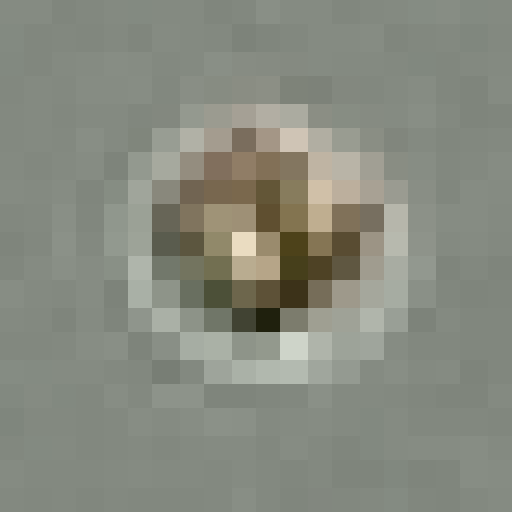
\includegraphics[width=0.25\textwidth]{img/r_dying_cell_0003.png}}}%
    \qquad
    \subfloat[$t = 44$]{{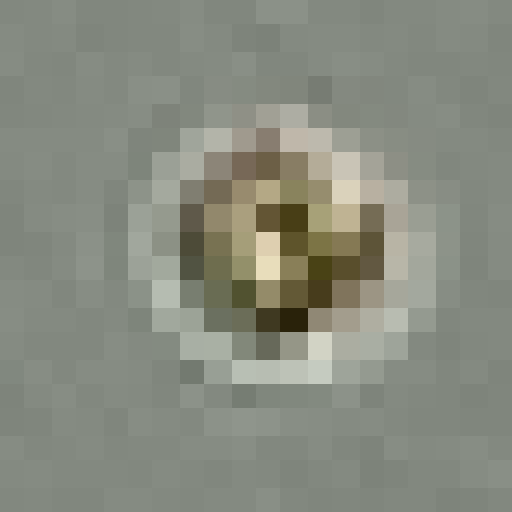
\includegraphics[width=0.25\textwidth]{img/r_dying_cell_0004.png}}}%
    \qquad
    \subfloat[$t = 92$]{{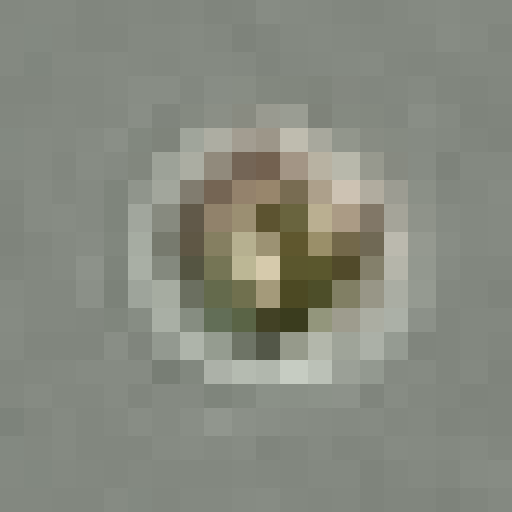
\includegraphics[width=0.25\textwidth]{img/r_dying_cell_0005.png}}}%
    \caption{An application of a neural algorithm of artistic style to phase contrast images of CAR-T cells (a) and a style source image (b) to synthesise a new image combining their characteristics in a ``simulated'' image (c).}%
    \label{fig:dying_cell_frames}
\end{figure}

\section{Blob detection Chapter 4}

\begin{figure}[h!]
\centering
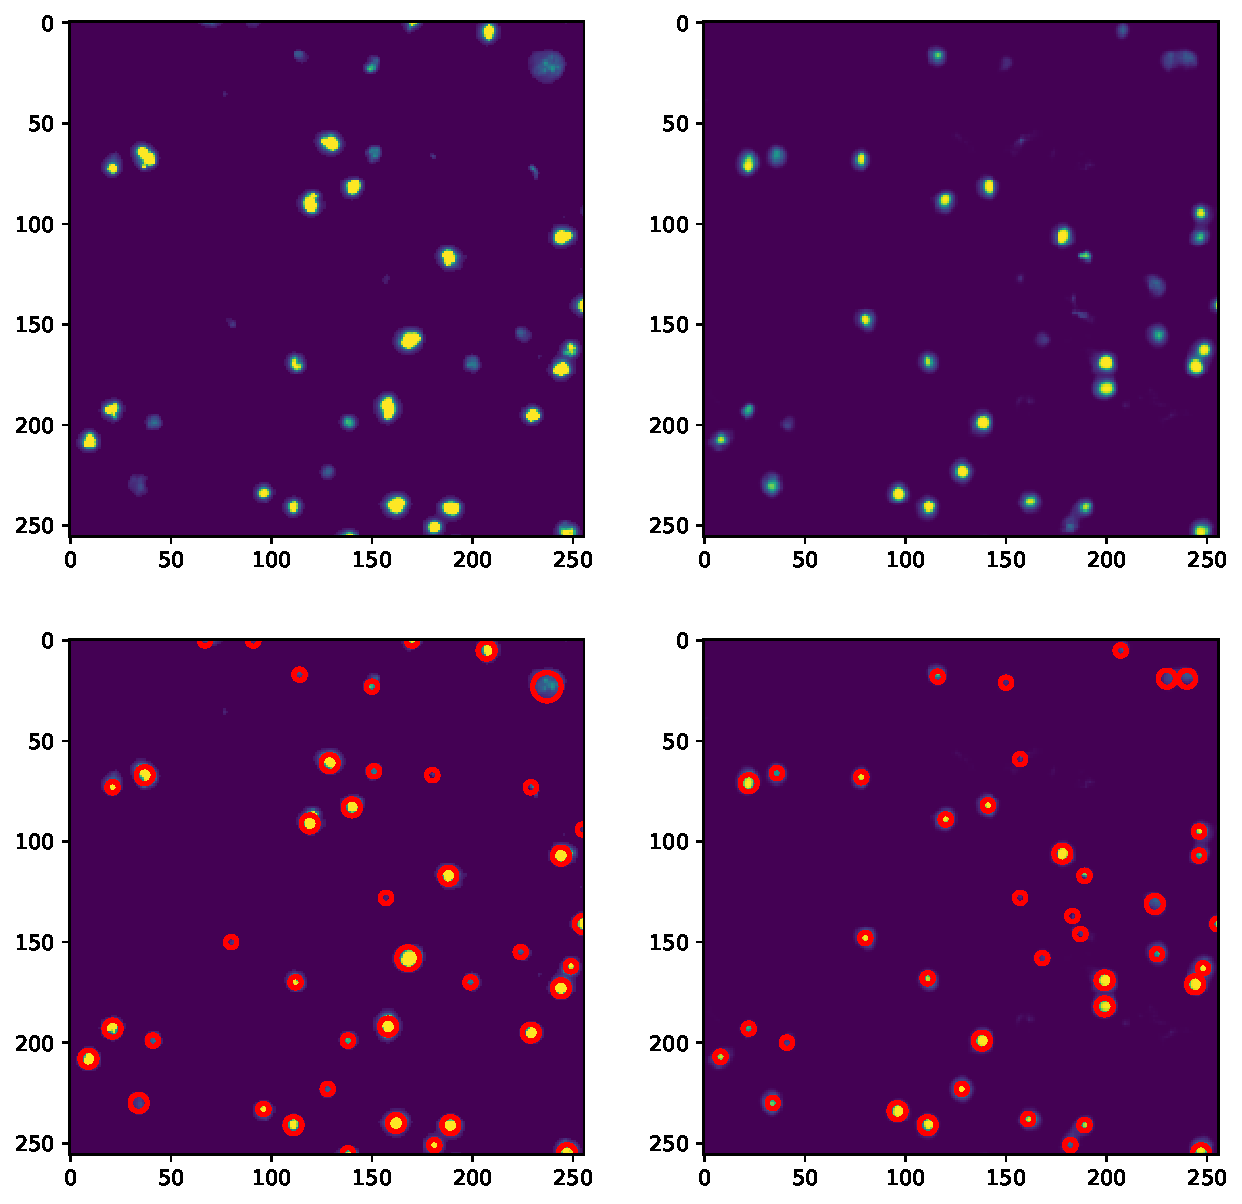
\includegraphics[width=0.85\textwidth]{img/blob_detection.pdf}
\caption{True positives: 31, False positives: 9, False negatives: 11}
\label{fig:blob_detection}
\end{figure}

\section{Image processing pipeline Chapter 4}

\begin{figure}[h!]%
    \centering
    \subfloat[mCherry and GFP fluorescence (left and center) and phase contrast signals (right) at $t = 0$]{{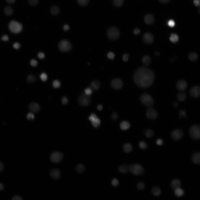
\includegraphics[width=0.25\textwidth]{img/pipeline_r.png} }}%
    \qquad
    \subfloat[mCherry and GFP fluorescence (left and center) and phase contrast signals (right) at $t = 70$]{{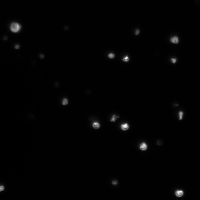
\includegraphics[width=0.25\textwidth]{img/pipeline_g} }}%
    \qquad
    \subfloat[mCherry and GFP fluorescence (left and center) and phase contrast signals (right) at $t = 70$]{{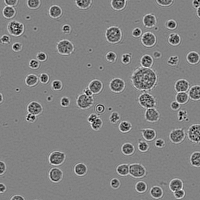
\includegraphics[width=0.25\textwidth]{img/pipeline_b.png} }}
    \qquad
    \subfloat[mCherry and GFP fluorescence (left and center) and phase contrast signals (right) at $t = 0$]{{
\includegraphics[width=0.25\textwidth]{img/pipeline_segmentation_bg.png} }}%
    \qquad
    \subfloat[mCherry and GFP fluorescence (left and center) and phase contrast signals (right) at $t = 70$]{{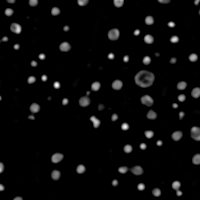
\includegraphics[width=0.25\textwidth]{img/pipeline_seg.png} }}%
    \qquad
    \subfloat[mCherry and GFP fluorescence (left and center) and phase contrast signals (right) at $t = 70$]{{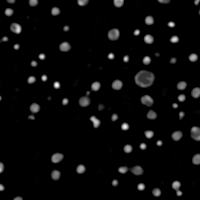
\includegraphics[width=0.25\textwidth]{img/pipeline_fill.png} }}
    \qquad
    \subfloat[mCherry and GFP fluorescence (left and center) and phase contrast signals (right) at $t = 0$]{{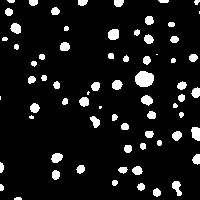
\includegraphics[width=0.25\textwidth]{img/pipeline_mask.png} }}%
    \qquad
    \subfloat[mCherry and GFP fluorescence (left and center) and phase contrast signals (right) at $t = 70$]{{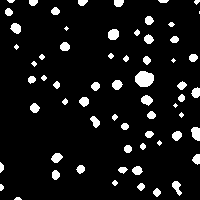
\includegraphics[width=0.25\textwidth]{img/pipeline_opened.png} }}%
    \qquad
    \subfloat[mCherry and GFP fluorescence (left and center) and phase contrast signals (right) at $t = 70$]{{
\includegraphics[width=0.25\textwidth]{img/pipeline_labels.png} }}
    \caption{Comparison of crops of the same cell population at times (a) $t = 0$ and (b) $t = 70$. Mitosis has brought about agglomerations of cells that are difficult to separate. The problem is exacerbated by a loss of fluorescence ``signal quenching'' over time.}%
    \label{fig:ground_truth_pipeline_example}%
\end{figure}
